\documentclass{standalone}
\usepackage{tikz}
\usetikzlibrary{patterns, positioning}


\begin{document}
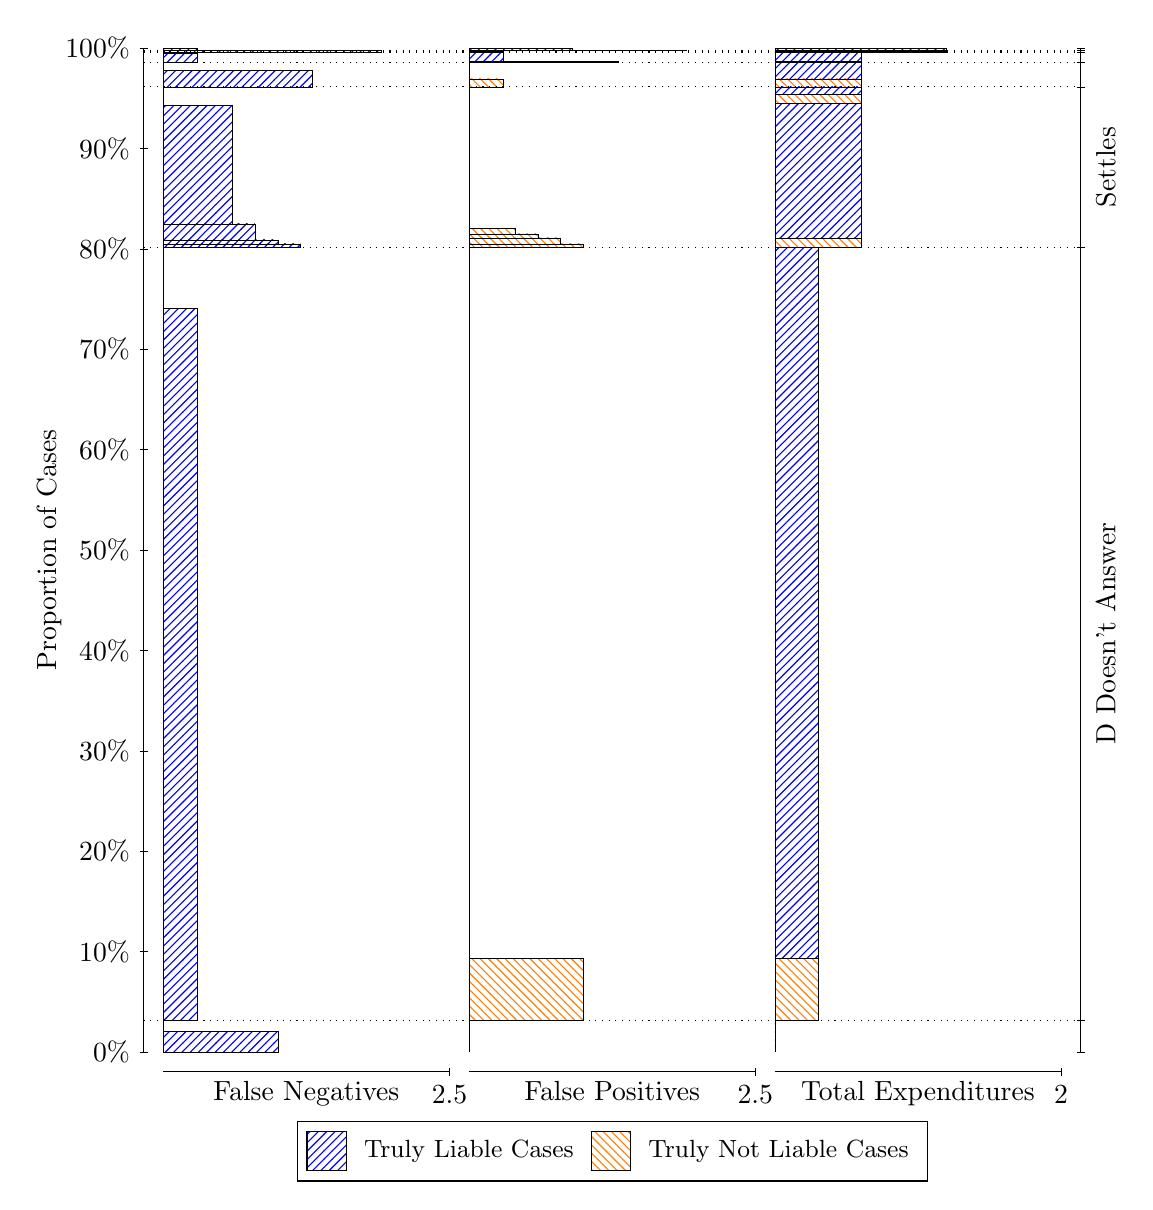
\begin{tikzpicture}
\draw[black, very thin] (1.5,1.75) -- (1.5,14.5);
\node[rotate=90, text=black, anchor=center] at (0.3, 8.125) {Proportion of Cases};
\draw[black, very thin] (1.45,1.75) -- (1.55,1.75);
\node[text=black, anchor=east] at (1.45, 1.75) {0\%};
\draw[black, very thin] (1.45,3.025) -- (1.55,3.025);
\node[text=black, anchor=east] at (1.45, 3.025) {10\%};
\draw[black, very thin] (1.45,4.3) -- (1.55,4.3);
\node[text=black, anchor=east] at (1.45, 4.3) {20\%};
\draw[black, very thin] (1.45,5.575) -- (1.55,5.575);
\node[text=black, anchor=east] at (1.45, 5.575) {30\%};
\draw[black, very thin] (1.45,6.85) -- (1.55,6.85);
\node[text=black, anchor=east] at (1.45, 6.85) {40\%};
\draw[black, very thin] (1.45,8.125) -- (1.55,8.125);
\node[text=black, anchor=east] at (1.45, 8.125) {50\%};
\draw[black, very thin] (1.45,9.4) -- (1.55,9.4);
\node[text=black, anchor=east] at (1.45, 9.4) {60\%};
\draw[black, very thin] (1.45,10.675) -- (1.55,10.675);
\node[text=black, anchor=east] at (1.45, 10.675) {70\%};
\draw[black, very thin] (1.45,11.95) -- (1.55,11.95);
\node[text=black, anchor=east] at (1.45, 11.95) {80\%};
\draw[black, very thin] (1.45,13.225) -- (1.55,13.225);
\node[text=black, anchor=east] at (1.45, 13.225) {90\%};
\draw[black, very thin] (1.45,14.5) -- (1.55,14.5);
\node[text=black, anchor=east] at (1.45, 14.5) {100\%};

\draw[black, very thin] (13.4,1.75) -- (13.4,14.5);
\draw[black, very thin] (13.35,1.75) -- (13.45,1.75);
\node[anchor=west] at (13.35, 1.75) {};
\draw[black, very thin] (13.35,2.1525) -- (13.45,2.1525);
\node[anchor=west] at (13.35, 2.1525) {};
\draw[black, very thin] (13.35,11.972) -- (13.45,11.972);
\node[anchor=west] at (13.35, 11.972) {};
\draw[black, very thin] (13.35,14.006) -- (13.45,14.006);
\node[anchor=west] at (13.35, 14.006) {};
\draw[black, very thin] (13.35,14.317) -- (13.45,14.317);
\node[anchor=west] at (13.35, 14.317) {};
\draw[black, very thin] (13.35,14.449) -- (13.45,14.449);
\node[anchor=west] at (13.35, 14.449) {};
\draw[black, very thin] (13.35,14.47) -- (13.45,14.47);
\node[anchor=west] at (13.35, 14.47) {};
\draw[black, very thin] (13.35,14.5) -- (13.45,14.5);
\node[anchor=west] at (13.35, 14.5) {};

\draw[black, very thin, pattern color=blue, pattern=north east lines] (1.75,1.75) rectangle (3.2033,2.0123);
\draw[black, very thin, pattern color=orange, pattern=north west lines] (1.75,2.0123) rectangle (1.75,2.1525);
\draw[black, very thin, pattern color=blue, pattern=north east lines] (1.75,2.1525) rectangle (2.186,11.19);
\draw[black, very thin, pattern color=orange, pattern=north west lines] (1.75,11.19) rectangle (1.75,11.972);
\draw[black, very thin, pattern color=blue, pattern=north east lines] (1.75,11.972) rectangle (3.494,12.013);
\draw[black, very thin, pattern color=blue, pattern=north east lines] (1.75,12.013) rectangle (3.2033,12.062);
\draw[black, very thin, pattern color=blue, pattern=north east lines] (1.75,12.062) rectangle (2.9127,12.267);
\draw[black, very thin, pattern color=blue, pattern=north east lines] (1.75,12.267) rectangle (2.622,13.771);
\draw[black, very thin, pattern color=orange, pattern=north west lines] (1.75,13.771) rectangle (1.75,14.006);
\draw[black, very thin, pattern color=blue, pattern=north east lines] (1.75,14.006) rectangle (3.6393,14.216);
\draw[black, very thin, pattern color=orange, pattern=north west lines] (1.75,14.216) rectangle (1.75,14.317);
\draw[black, very thin, pattern color=blue, pattern=north east lines] (1.75,14.317) rectangle (2.186,14.438);
\draw[black, very thin, pattern color=orange, pattern=north west lines] (1.75,14.438) rectangle (1.75,14.449);
\draw[black, very thin, pattern color=blue, pattern=north east lines] (1.75,14.449) rectangle (4.5113,14.466);
\draw[black, very thin, pattern color=orange, pattern=north west lines] (1.75,14.466) rectangle (1.75,14.47);
\draw[black, very thin, pattern color=blue, pattern=north east lines] (1.75,14.47) rectangle (2.186,14.498);
\draw[black, very thin, pattern color=orange, pattern=north west lines] (1.75,14.498) rectangle (1.75,14.5);
\draw[black, very thin, pattern color=orange, pattern=north west lines] (5.6333,1.75) rectangle (5.6333,1.8902);
\draw[black, very thin, pattern color=blue, pattern=north east lines] (5.6333,1.8902) rectangle (5.6333,2.1525);
\draw[black, very thin, pattern color=orange, pattern=north west lines] (5.6333,2.1525) rectangle (7.0867,2.9346);
\draw[black, very thin, pattern color=blue, pattern=north east lines] (5.6333,2.9346) rectangle (5.6333,11.972);
\draw[black, very thin, pattern color=orange, pattern=north west lines] (5.6333,11.972) rectangle (7.0867,12.013);
\draw[black, very thin, pattern color=orange, pattern=north west lines] (5.6333,12.013) rectangle (6.796,12.09);
\draw[black, very thin, pattern color=orange, pattern=north west lines] (5.6333,12.09) rectangle (6.5053,12.141);
\draw[black, very thin, pattern color=orange, pattern=north west lines] (5.6333,12.141) rectangle (6.2147,12.207);
\draw[black, very thin, pattern color=blue, pattern=north east lines] (5.6333,12.207) rectangle (5.6333,14.006);
\draw[black, very thin, pattern color=orange, pattern=north west lines] (5.6333,14.006) rectangle (6.0693,14.107);
\draw[black, very thin, pattern color=blue, pattern=north east lines] (5.6333,14.107) rectangle (5.6333,14.317);
\draw[black, very thin, pattern color=orange, pattern=north west lines] (5.6333,14.317) rectangle (7.5227,14.328);
\draw[black, very thin, pattern color=blue, pattern=north east lines] (5.6333,14.328) rectangle (6.0693,14.449);
\draw[black, very thin, pattern color=orange, pattern=north west lines] (5.6333,14.449) rectangle (6.0693,14.454);
\draw[black, very thin, pattern color=blue, pattern=north east lines] (5.6333,14.454) rectangle (5.6333,14.47);
\draw[black, very thin, pattern color=orange, pattern=north west lines] (5.6333,14.47) rectangle (8.3947,14.472);
\draw[black, very thin, pattern color=blue, pattern=north east lines] (5.6333,14.472) rectangle (6.9413,14.5);
\draw[black, very thin, pattern color=orange, pattern=north west lines] (9.5167,1.75) rectangle (9.5167,1.8902);
\draw[black, very thin, pattern color=blue, pattern=north east lines] (9.5167,1.8902) rectangle (9.5167,2.1525);
\draw[black, very thin, pattern color=orange, pattern=north west lines] (9.5167,2.1525) rectangle (10.062,2.9346);
\draw[black, very thin, pattern color=blue, pattern=north east lines] (9.5167,2.9346) rectangle (10.062,11.972);
\draw[black, very thin, pattern color=orange, pattern=north west lines] (9.5167,11.972) rectangle (10.607,12.09);
\draw[black, very thin, pattern color=blue, pattern=north east lines] (9.5167,12.09) rectangle (10.607,13.799);
\draw[black, very thin, pattern color=orange, pattern=north west lines] (9.5167,13.799) rectangle (10.607,13.916);
\draw[black, very thin, pattern color=blue, pattern=north east lines] (9.5167,13.916) rectangle (10.607,14.006);
\draw[black, very thin, pattern color=orange, pattern=north west lines] (9.5167,14.006) rectangle (10.607,14.107);
\draw[black, very thin, pattern color=blue, pattern=north east lines] (9.5167,14.107) rectangle (10.607,14.317);
\draw[black, very thin, pattern color=orange, pattern=north west lines] (9.5167,14.317) rectangle (10.607,14.328);
\draw[black, very thin, pattern color=blue, pattern=north east lines] (9.5167,14.328) rectangle (10.607,14.449);
\draw[black, very thin, pattern color=orange, pattern=north west lines] (9.5167,14.449) rectangle (11.697,14.454);
\draw[black, very thin, pattern color=blue, pattern=north east lines] (9.5167,14.454) rectangle (11.697,14.47);
\draw[black, very thin, pattern color=orange, pattern=north west lines] (9.5167,14.47) rectangle (11.697,14.472);
\draw[black, very thin, pattern color=blue, pattern=north east lines] (9.5167,14.472) rectangle (11.697,14.5);
\draw[black, dotted] (1.5,2.1525) -- (13.4,2.1525);
\draw[black, dotted] (1.5,11.972) -- (13.4,11.972);
\draw[black, dotted] (1.5,14.006) -- (13.4,14.006);
\draw[black, dotted] (1.5,14.317) -- (13.4,14.317);
\draw[black, dotted] (1.5,14.449) -- (13.4,14.449);
\draw[black, dotted] (1.5,14.47) -- (13.4,14.47);
\draw[black, very thin] (1.75,1.5) -- (5.3833,1.5);
\node[text=black, anchor=north] at (3.5667, 1.5) {False Negatives};
\draw[black, very thin] (5.3833,1.45) -- (5.3833,1.55);
\node[text=black, anchor=north] at (5.3833, 1.45) {2.5};

\draw[black, very thin] (5.6333,1.5) -- (9.2667,1.5);
\node[text=black, anchor=north] at (7.45, 1.5) {False Positives};
\draw[black, very thin] (9.2667,1.45) -- (9.2667,1.55);
\node[text=black, anchor=north] at (9.2667, 1.45) {2.5};

\draw[black, very thin] (9.5167,1.5) -- (13.15,1.5);
\node[text=black, anchor=north] at (11.333, 1.5) {Total Expenditures};
\draw[black, very thin] (13.15,1.45) -- (13.15,1.55);
\node[text=black, anchor=north] at (13.15, 1.45) {2};


\node[text=black, centered, rotate=90] at (13.72, 7.0625) {D Doesn't Answer};
\node[text=black, centered, rotate=90] at (13.72, 12.989) {Settles};





\draw (7.449999999999999,1.5) node[draw=none] (baseCoordinate) {};
\begin{scope}[align=center]
        \matrix[scale=0.5, draw=black, below=0.5cm of baseCoordinate, nodes={draw}, column sep=0.1cm]{
            \node[rectangle, draw, minimum width=0.5cm, minimum height=0.5cm, pattern color=blue, pattern=north east lines] {}; &
            \node[draw=none, font=\small, text=black] (B) {Truly Liable Cases}; &
            \node[rectangle, draw, minimum width=0.5cm, minimum height=0.5cm, pattern color=orange, pattern=north west lines] {}; &
            \node[draw=none, font=\small, text=black] (B) {Truly Not Liable Cases}; \\
            };
\end{scope}

\end{tikzpicture}
\end{document}